\section{Casi d'uso\textsubscript{G}}

\subsection{Obiettivi}
La sezione 3 Casi d'uso\textsubscript{G} ha come obiettivo l'identificazione e la descrizione di tutti i casi d'uso\textsubscript{G}, ovvero interazioni tra sistema ed attori\textsubscript{G}, individuati dagli analisti nel tempo tramite lo studio del capitolato d'appalto, del dominio\textsubscript{G}, e tramite incontri con il committente.

\subsection{Attori\textsubscript{G}}
Dato che il requisito obbligatorio richiede la costruzione di una pagina di login che presenti un sistema in grado di distinguere un utente umano da un robot, il prodotto presenterà due tipologie principali di attori\textsubscript{G}:
\begin{figure}[H]
    \centering
    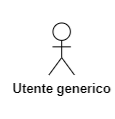
\includegraphics[scale = 1]{img/utente_generico.png}\\
    \caption{Utente generico}
\end{figure}
L'utente generico, che potrà essere una persona fisica o anche un bot\textsubscript{G}, potrà accedere alle funzionalità della WebApp. \\
\begin{figure}[H]
    \centering
    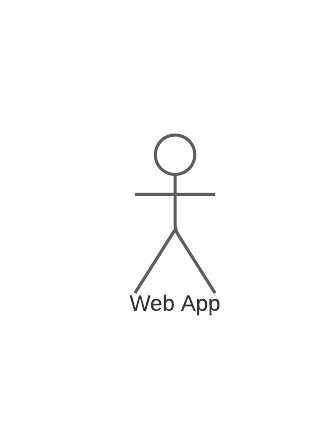
\includegraphics[scale = 0.8]{img/webapp.png}\\
    \caption{Utente WebApp}
\end{figure}
La WebApp, che potrà accedere alle funzionalità offerte dal servizio CAPTCHA\textsubscript{G}. \\

\subsection{WebApp}

\begin{figure}[H]
    \centering
    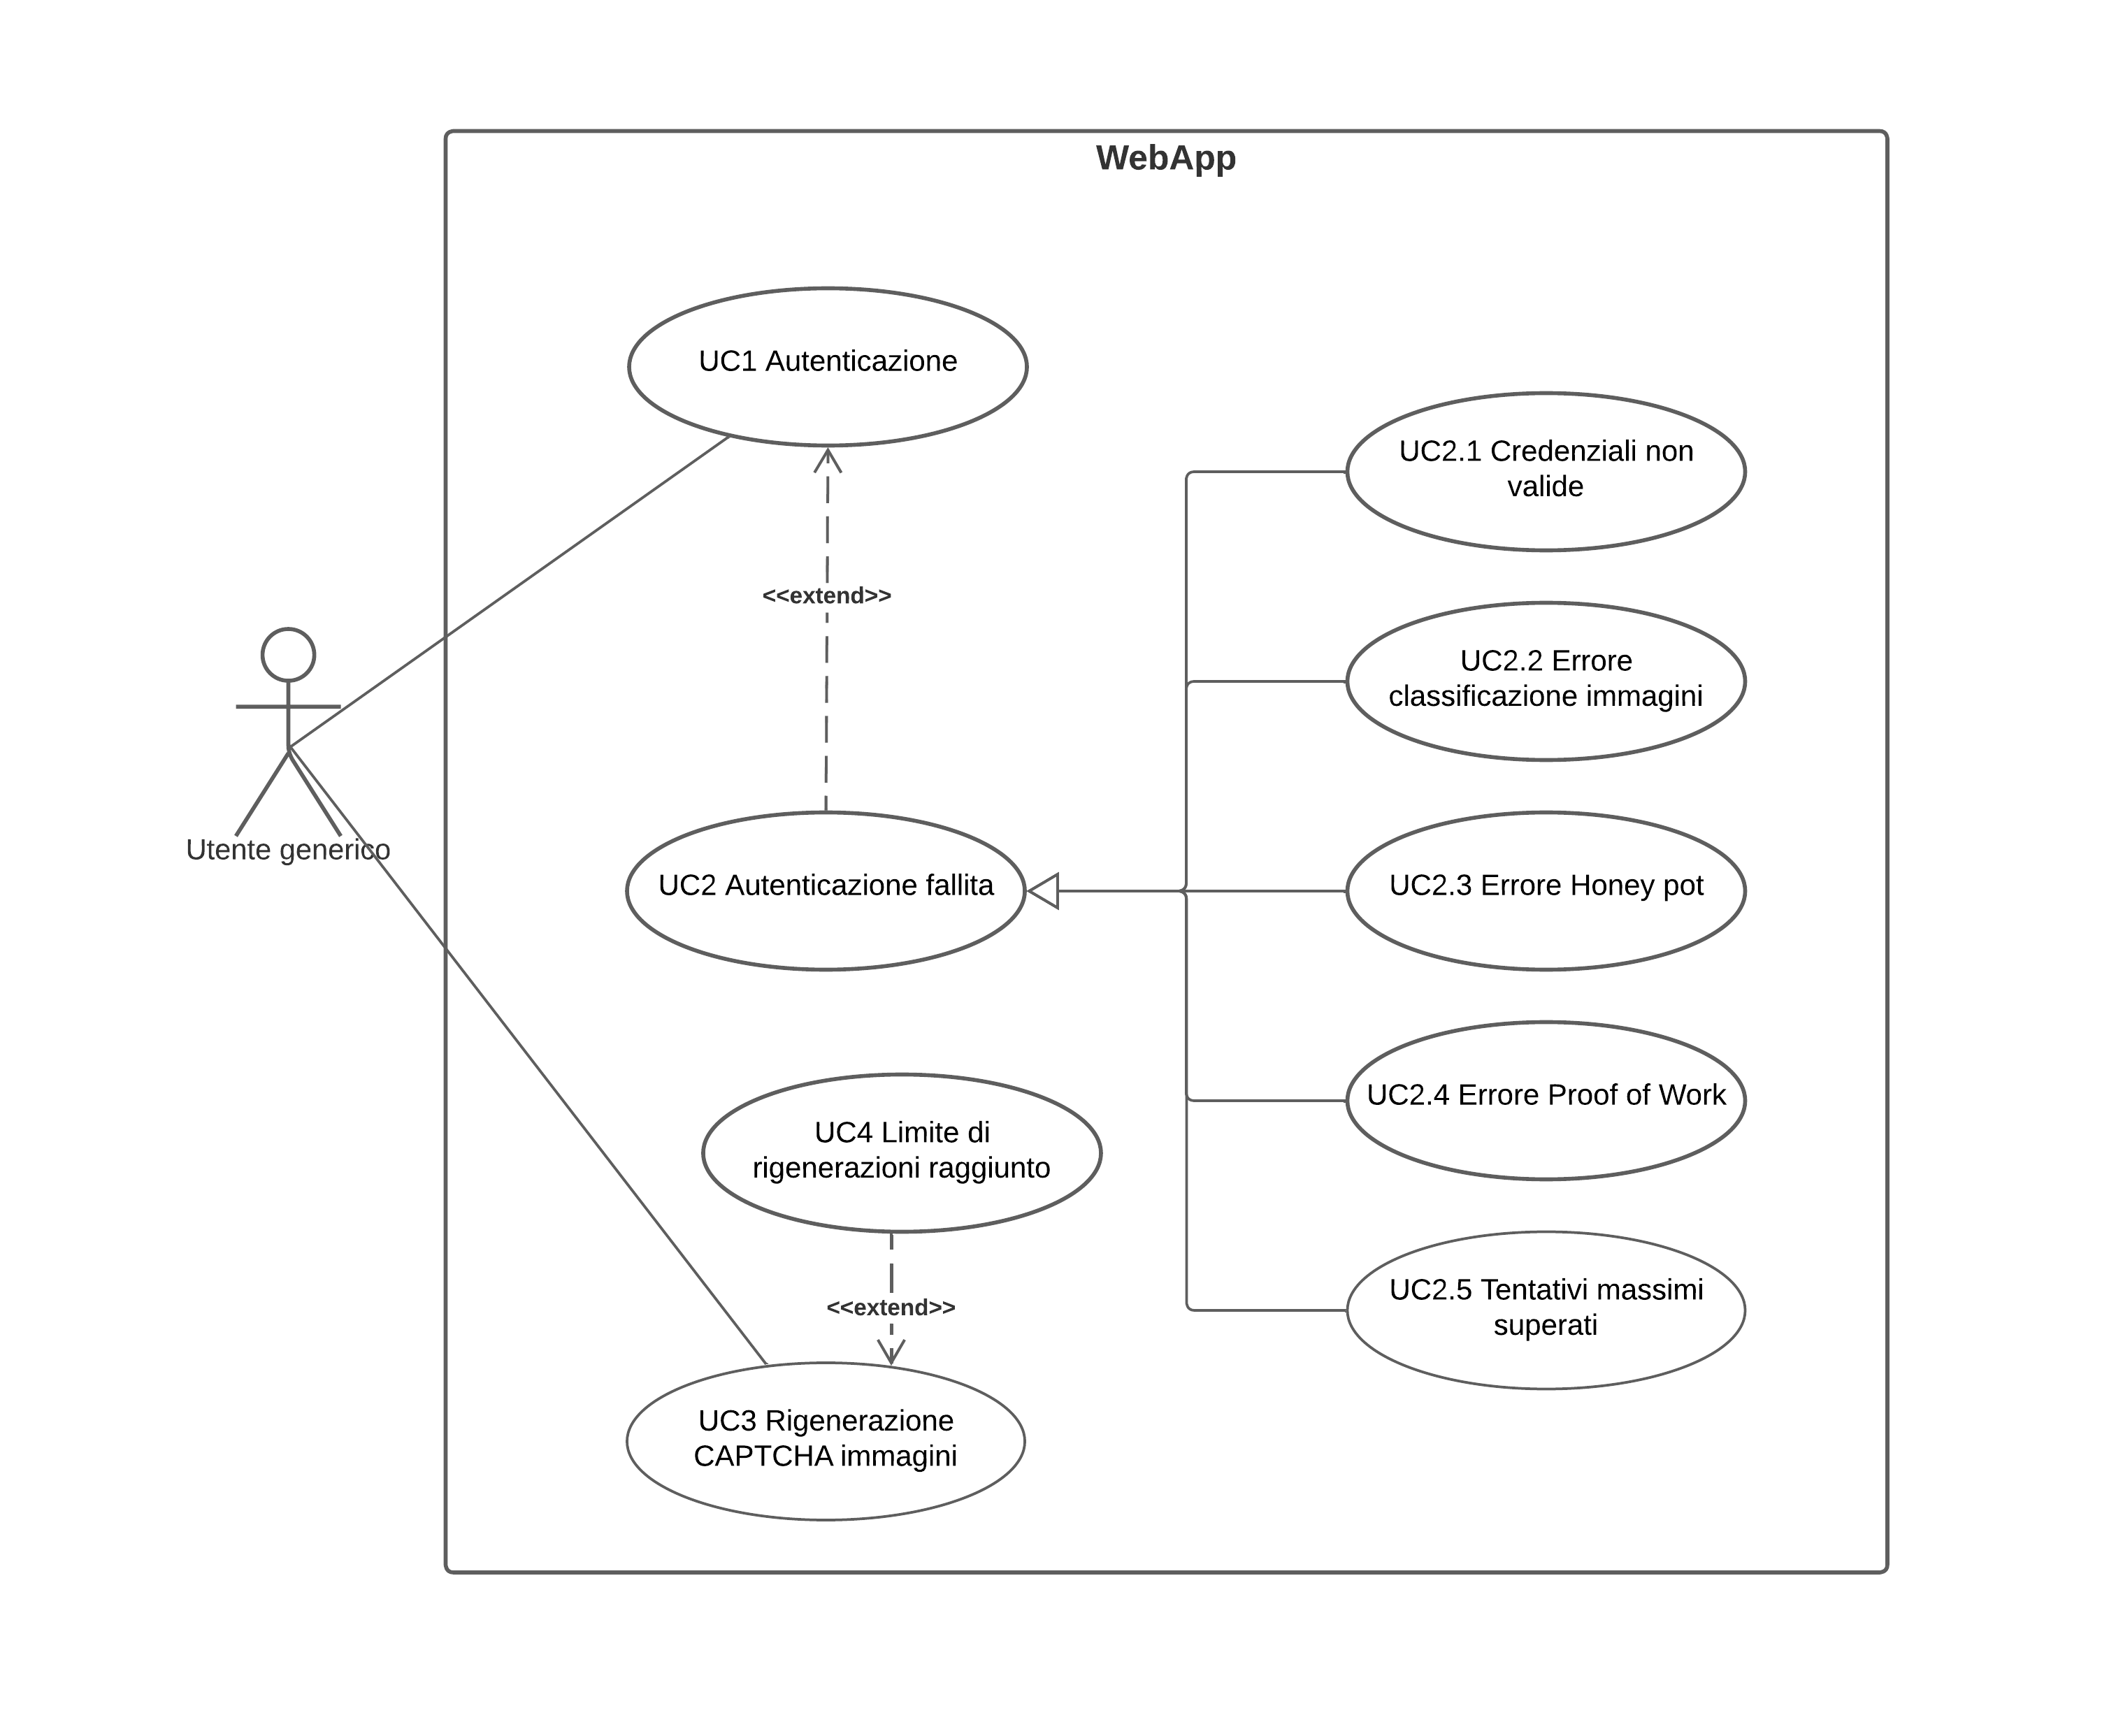
\includegraphics[scale=0.6]{img/web_app.png}
    \caption{Webapp}
\end{figure}

\begin{figure}[H]
    \centering
    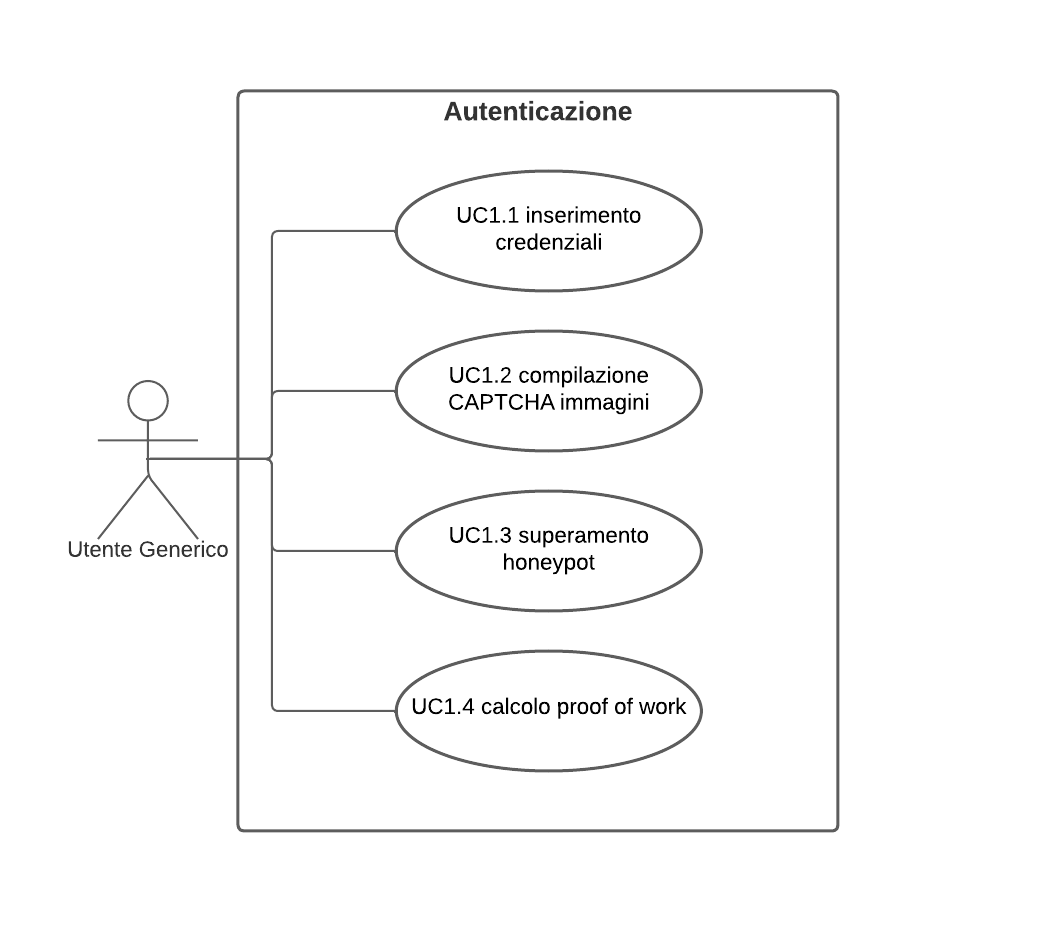
\includegraphics[scale=0.8]{img/Autenticazione.png}
    \caption{UC1 Autenticazione}
\end{figure}

\subsubsection{UC1 - Autenticazione}
\textbf{Attore primario}: Utente generico.\\
\textbf{Precondizioni}: Il sistema non riconosce l'utente.\\
\textbf{Postcondizioni}: L'utente è autenticato nel sistema.\\

\textbf{Scenario principale}: L'utente:
\begin{enumerate}
\item Inserisce le credenziali d'accesso [UC1.1];
\item Compila il CAPTCHA\textsubscript{G} immagini [UC1.2];
\item Supera l'honeypot\textsubscript{G} [UC1.3];
\item Calcola il proof of work\textsubscript{G} [UC1.4].
\end{enumerate}

\textbf{Scenari alternativi}:
\begin{enumerate}
    \item L’utente non supera l'autenticazione [UC2].
\end{enumerate}

\begin{figure}[H]
    \centering
    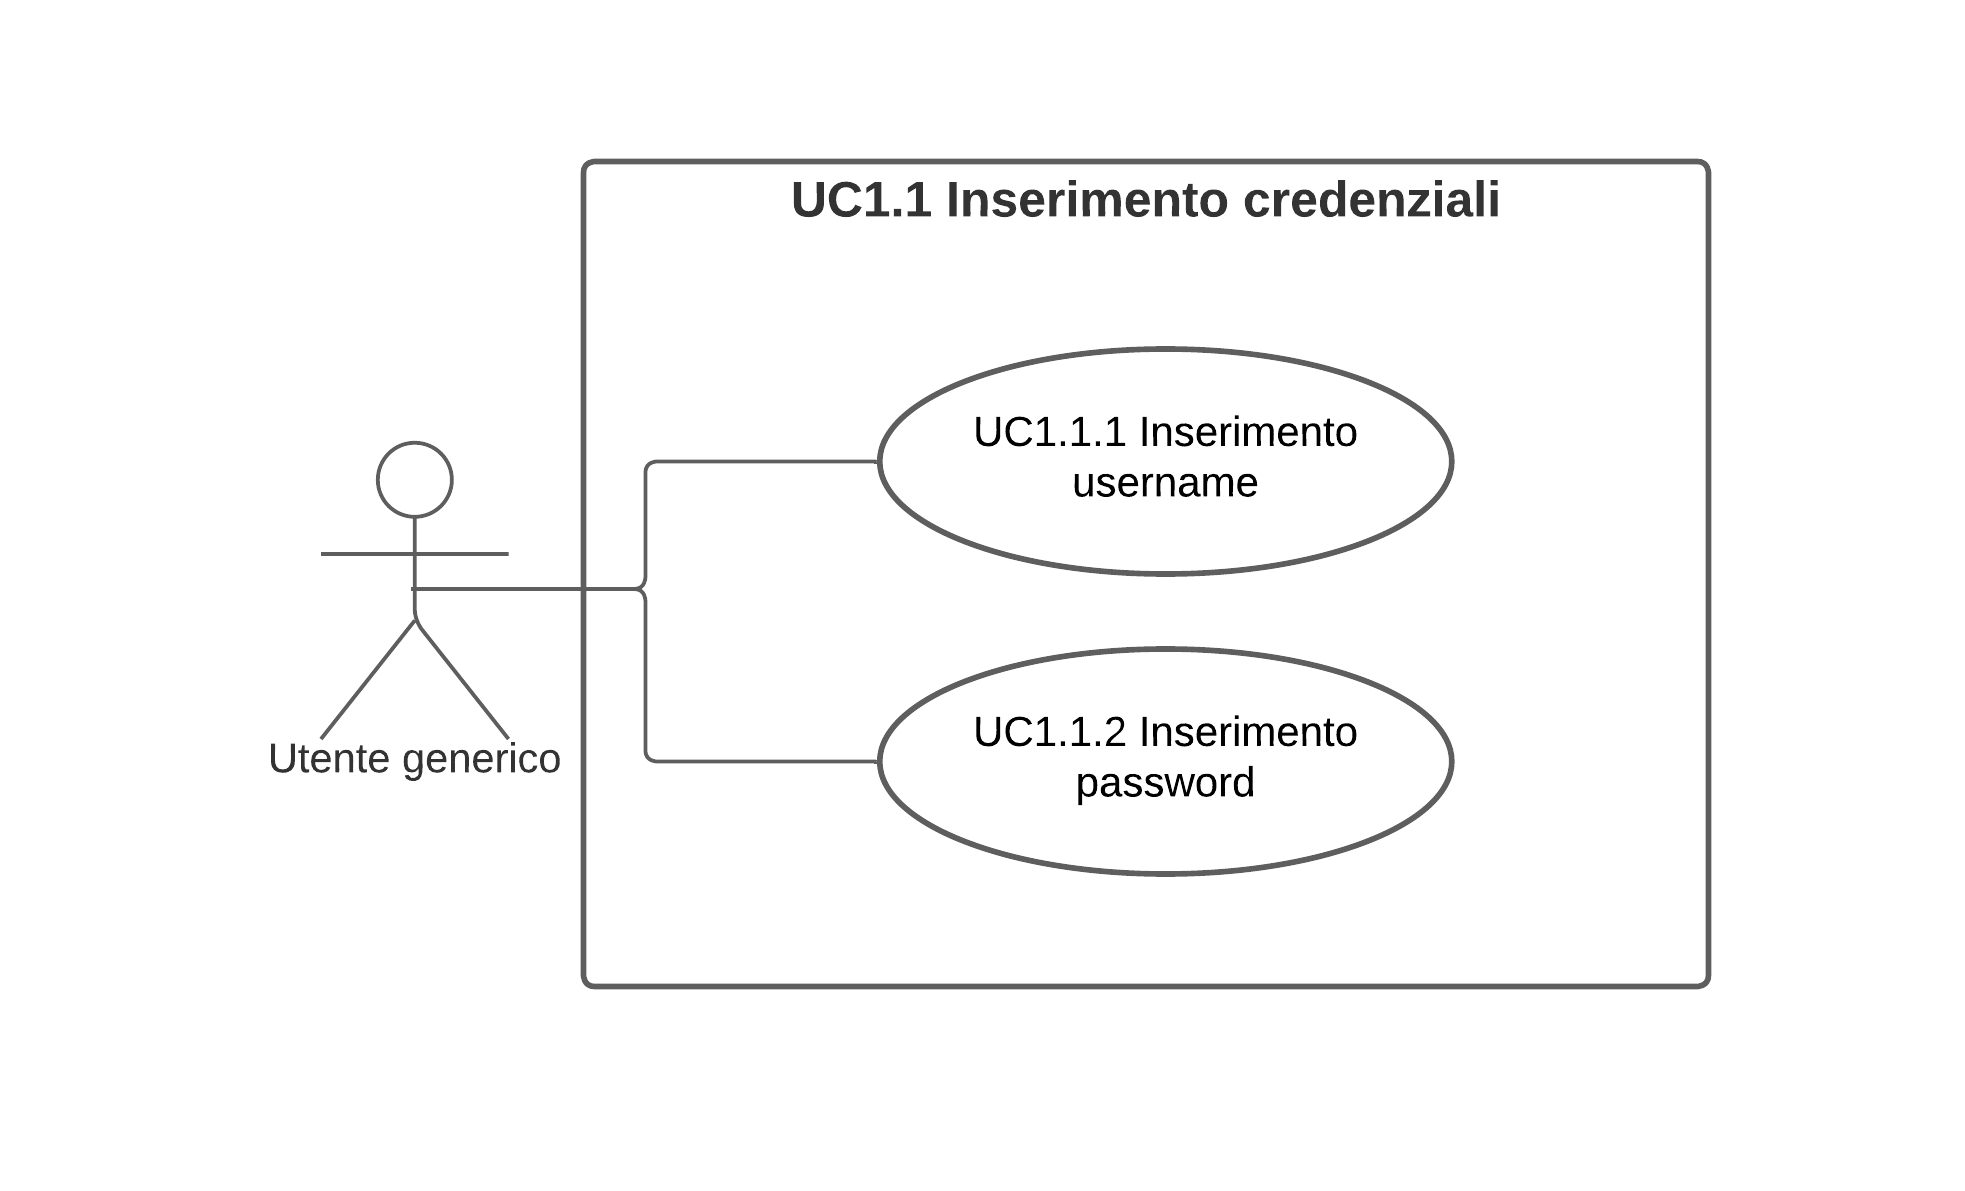
\includegraphics[scale=0.8]{img/inserimento_credenziali.png}
    \caption{UC1.1 Inserimento credenziali}
\end{figure}

\paragraph{UC1.1 - Inserimento credenziali}
\textbf{Attore primario}: Utente generico.\\
\textbf{Precondizioni}: Il sistema non riconosce l'utente.\\
\textbf{Postcondizioni}: Il sistema ha ricevuto le credenziali dell'utente.\\

\textbf{Scenario principale}: L'utente:
\begin{enumerate}
   \item Inserisce il proprio username [UC1.1.1];
   \item Inserisce la propria password [UC1.1.2].
\end{enumerate}

\subparagraph{UC1.1.1 - } \textbf{Inserimento username}\\
\textbf{Attore primario}: Utente generico.\\
\textbf{Precondizioni}: L'username non è stata inserita.\\
\textbf{Postcondizioni}: Il sistema ha ricevuto lo username dell'utente.\\

\textbf{Scenario principale}: L'utente:
\begin{enumerate}
   \item Inserisce il proprio username.
\end{enumerate}

\subparagraph{UC1.1.2 - } \textbf{Inserimento password} \\
\textbf{Attore primario}: Utente generico.\\
\textbf{Precondizioni}: La password non è stata inserita.\\
\textbf{Postcondizioni}: Il sistema ha ricevuto la password dell'utente.\\

\textbf{Scenario principale}: L'utente:
\begin{enumerate}
   \item Inserisce la propria password.
\end{enumerate}

\paragraph{UC1.2 - Compilazione CAPTCHA\textsubscript{G} immagini}
\textbf{Attore primario}: Utente generico.\\
\textbf{Precondizioni}: L'utente visualizza il CAPTCHA\textsubscript{G} immagini proposto dal sistema.\\
\textbf{Postcondizioni}: L'utente ha risolto il CAPTCHA\textsubscript{G} immagini, non necessariamente in modo corretto.\\

\textbf{Scenario principale}: L'utente:
\begin{enumerate}
   \item Visualizza le immagini distorte appartenenti al CAPTCHA\textsubscript{G};
   \item Classifica le immagini visualizzate secondo il proprio giudizio, che può non corrispondere totalmente alla classificazione in uso dal sistema.
\end{enumerate}

\paragraph{UC1.3 - Superamento honeypot\textsubscript{G}}
\textbf{Attore primario}: Utente generico.\\
\textbf{Precondizioni}: All'utente viene presentata una trappola honeypot\textsubscript{G}.\\
\textbf{Postcondizioni}: L'utente supera l'honeypot\textsubscript{G}.\\

\textbf{Scenario principale}:
\begin{enumerate}
   \item All'utente viene presentata una trappola honeypot\textsubscript{G}, sottoforma di immagine nascosta ad un utente umano, ma visibile ad un bot\textsubscript{G};
   \item L'utente non seleziona l'immagine nascosta.
\end{enumerate}

\paragraph{UC1.4 - Calcolo proof of work\textsubscript{G}}
\textbf{Attore primario}: Utente generico.\\
\textbf{Precondizioni}: All'utente viene richiesto il calcolo del proof of work\textsubscript{G}.\\
\textbf{Postcondizioni}: Il proof of work\textsubscript{G} viene calcolato.\\

\textbf{Scenario principale}:
\begin{enumerate}
   \item Viene calcolato il proof of work\textsubscript{G};
   \item Il risultato viene fornito al sistema.
\end{enumerate}

\subsubsection{UC2 - Autenticazione fallita}
\textbf{Attore primario}: Utente generico.\\
\textbf{Precondizioni}: L’utente ha commesso un errore durante l'autenticazione.\\
\textbf{Postcondizioni}: L’utente visualizza un messaggio di errore e l’operazione di autenticazione fallisce.\\

\textbf{Scenario principale}:
\begin{enumerate}
   \item L’utente commette un errore nella compilazione del modulo di login;
   \item L'utente visualizza un messaggio di errore;
   \item L'utente non viene autenticato nel sistema.
\end{enumerate}

\textbf{Generalizzazioni}: L'utente ha commesso uno dei seguenti errori:
\begin{enumerate}
	\item Ha inserito delle credenziali errate [UC2.1];
	\item Ha sbagliato la classificazione delle immagini [UC2.2];
	\item E' caduto nella trappola honeypot\textsubscript{G} [UC2.3];
	\item Non ha calcolato il proof of work\textsubscript{G} [UC2.4];
	\item Ha superato il numero massimo di tentativi disponibili [UC2.5].
\end{enumerate}

\paragraph{UC2.1 - Credenziali errate}
\textbf{Attore primario:} Utente generico.\\
\textbf{Precondizioni}: L’utente non ha inserito le credenziali corrette.\\
\textbf{Postcondizioni}: L’utente visualizza un messaggio di errore e l’operazione di autenticazione fallisce.\\

\textbf{Scenario principale}:
\begin{enumerate}
    \item L'utente inserisce credenziali non valide per l'autenticazione nel sistema;
	\item L’utente visualizza un messaggio di errore;
	\item Il numero di tentativi consecutivi compiuti dall’utente aumenta di 1.
\end{enumerate}

\textbf{Generalizzazioni}:
\begin{enumerate}
    \item L'utente inserisce un'username non valida per l'autenticazione [UC2.1.1];
	\item L'utente inserisce una password non valida per l'autenticazione [UC2.1.2].
\end{enumerate}

\subparagraph{UC2.1.1 - } \textbf{Username errata}\\
\textbf{Attore primario:} Utente generico.\\
\textbf{Precondizioni}: L’utente ha inserito un'username non valida per l'autenticazione.\\
\textbf{Postcondizioni}: L’utente visualizza un messaggio di errore e l’operazione di autenticazione fallisce.\\

\textbf{Scenario principale}:
\begin{enumerate}
    \item L'utente inserisce un'username non riconosciuta dal sistema, compresa la possibilità che l'username sia vuota;
	\item L’utente visualizza un messaggio di errore;
	\item Il numero di tentativi consecutivi compiuti dall’utente aumenta di 1.
\end{enumerate}

\subparagraph{UC2.1.2 - } \textbf{Password errata}\\
\textbf{Attore primario:} Utente generico.\\
\textbf{Precondizioni}: L’utente ha inserito una password non valida per l'autenticazione.\\
\textbf{Postcondizioni}: L’utente visualizza un messaggio di errore e l’operazione di autenticazione fallisce.\\

\textbf{Scenario principale}:
\begin{enumerate}
    \item L'utente inserisce una password non corretta per l'username scelta, compresa la possibilità che la password sia vuota;
	\item L’utente visualizza un messaggio di errore;
	\item Il numero di tentativi consecutivi compiuti dall’utente aumenta di 1.
\end{enumerate}

\paragraph{UC2.2 - Errore classificazione immagini}
\textbf{Attore primario:} Utente generico.\\
    \textbf{Precondizioni}: L’utente non ha compilato correttamente il CAPTCHA\textsubscript{G} immagini.\\
\textbf{Postcondizioni}: L’utente visualizza un messaggio di errore e l’operazione di autenticazione fallisce.\\

\textbf{Scenario principale}:
\begin{enumerate}
    \item L'utente classifica le immagini proposte superando il margine di errore tollerato rispetto alla classificazione in uso dal sistema;
	\item L’utente visualizza un messaggio di errore;
	\item Il numero di tentativi consecutivi compiuti dall’utente aumenta di 1.
\end{enumerate}

\paragraph{UC2.3 - Errore honeypot\textsubscript{G}}
\textbf{Attore primario:} Utente generico.\\
\textbf{Precondizioni}: L’utente ha selezionato l'immagine nascosta.\\
\textbf{Postcondizioni}: L’utente visualizza un messaggio di errore e l’operazione di autenticazione fallisce.\\

\textbf{Scenario principale}:
\begin{enumerate}
    \item L'utente seleziona l'immagine nascosta;
	\item L’utente visualizza un messaggio di errore;
	\item L'utente viene riconosciuto come bot\textsubscript{G} e verrà bloccato nei futuri tentativi di login.
\end{enumerate}

\paragraph{UC2.4 - Errore proof of work\textsubscript{G}}
\textbf{Attore primario:} Utente generico\\
\textbf{Precondizioni}: Il proof of work\textsubscript{G} non è stato calcolato.\\
\textbf{Postcondizioni}:  L’utente visualizza un messaggio di errore e l’operazione di autenticazione fallisce.\\

\textbf{Scenario principale}:
\begin{enumerate}
    \item In alternativa:
    \begin{itemize}
        \item L'utente inserisce le credenziali e compila il CAPTCHA\textsubscript{G} immagini in maniera troppo rapida, per cui non viene eseguito il calcolo del proof of work\textsubscript{G};
        \item L'utente invia un proof of work\textsubscript{G} non valido.
    \end{itemize}
	\item L’utente visualizza un messaggio di errore;
	\item L'utente viene bloccato in fase di login.
\end{enumerate}

\paragraph{UC2.5 - Tentativi massimi superati}
\textbf{Attore primario:} Utente generico.\\
\textbf{Precondizioni}: L'utente ha superato il numero massimo di tentativi consentiti per il login.\\
\textbf{Postcondizioni}: L’utente visualizza un messaggio di errore e l’operazione di autenticazione fallisce.\\

\textbf{Scenario principale}:
\begin{enumerate}
    \item L'utente effettua più tentativi di login consecutivi rispetto a quelli consentiti dal sistema;
	\item L’utente visualizza un messaggio di errore;
	\item L'utente potrà  riprovare ad autenticarsi più tardi.
\end{enumerate}

\subsubsection{UC3 - Rigenerazione CAPTCHA\textsubscript{G} immagini}
\textbf{Attore primario}: Utente generico.\\
\textbf{Precondizioni}: L'utente non riconosce le immagini contenute nel CAPTCHA\textsubscript{G} e pertanto non può procedere con la loro classificazione.\\
\textbf{Postcondizioni}: All'utente viene proposto un nuovo set di immagini da classificare.\\

\textbf{Scenario principale}:
\begin{enumerate}
   \item L'utente non è in grado di classificare le immagini proposte dal sistema;
   \item L'utente richiede un altro set di immagini;
   \item Il sistema genera un nuovo set di immagini e le propone all'utente;
   \item Il numero di rigenerazioni CAPTCHA\textsubscript{G} immagini richieste dall’utente aumenta di 1;
   \item L'utente può procedere con la risoluzione del CAPTCHA\textsubscript{G} immagini.
\end{enumerate}
\textbf{Scenari alternativi}:
\begin{enumerate}
   \item L'utente ha superato il numero massimo di richieste di rigenerazione CAPTCHA\textsubscript{G} immagini consentito [UC4].
\end{enumerate}

\subsubsection{UC4 - Limite di rigenerazioni aggiunto}
\textbf{Attore primario:} Utente generico.\\
\textbf{Precondizioni}: L'utente ha superato il numero massimo di richieste di rigenerazione CAPTCHA\textsubscript{G} immagini consentito.\\
\textbf{Postcondizioni}: L’utente visualizza un messaggio di errore e il CAPTCHA\textsubscript{G} immagini non viene rigenerato.\\

\textbf{Scenario principale}:
\begin{enumerate}
    \item L'utente effettua più richieste consecutive di rigenerazione CAPTCHA\textsubscript{G} immagini rispetto a quelle consentite dal sistema;
	\item L’utente visualizza un messaggio di errore.
\end{enumerate}

\subsection{CAPTCHA\textsubscript{G}}

\begin{figure}[H]
    \centering
    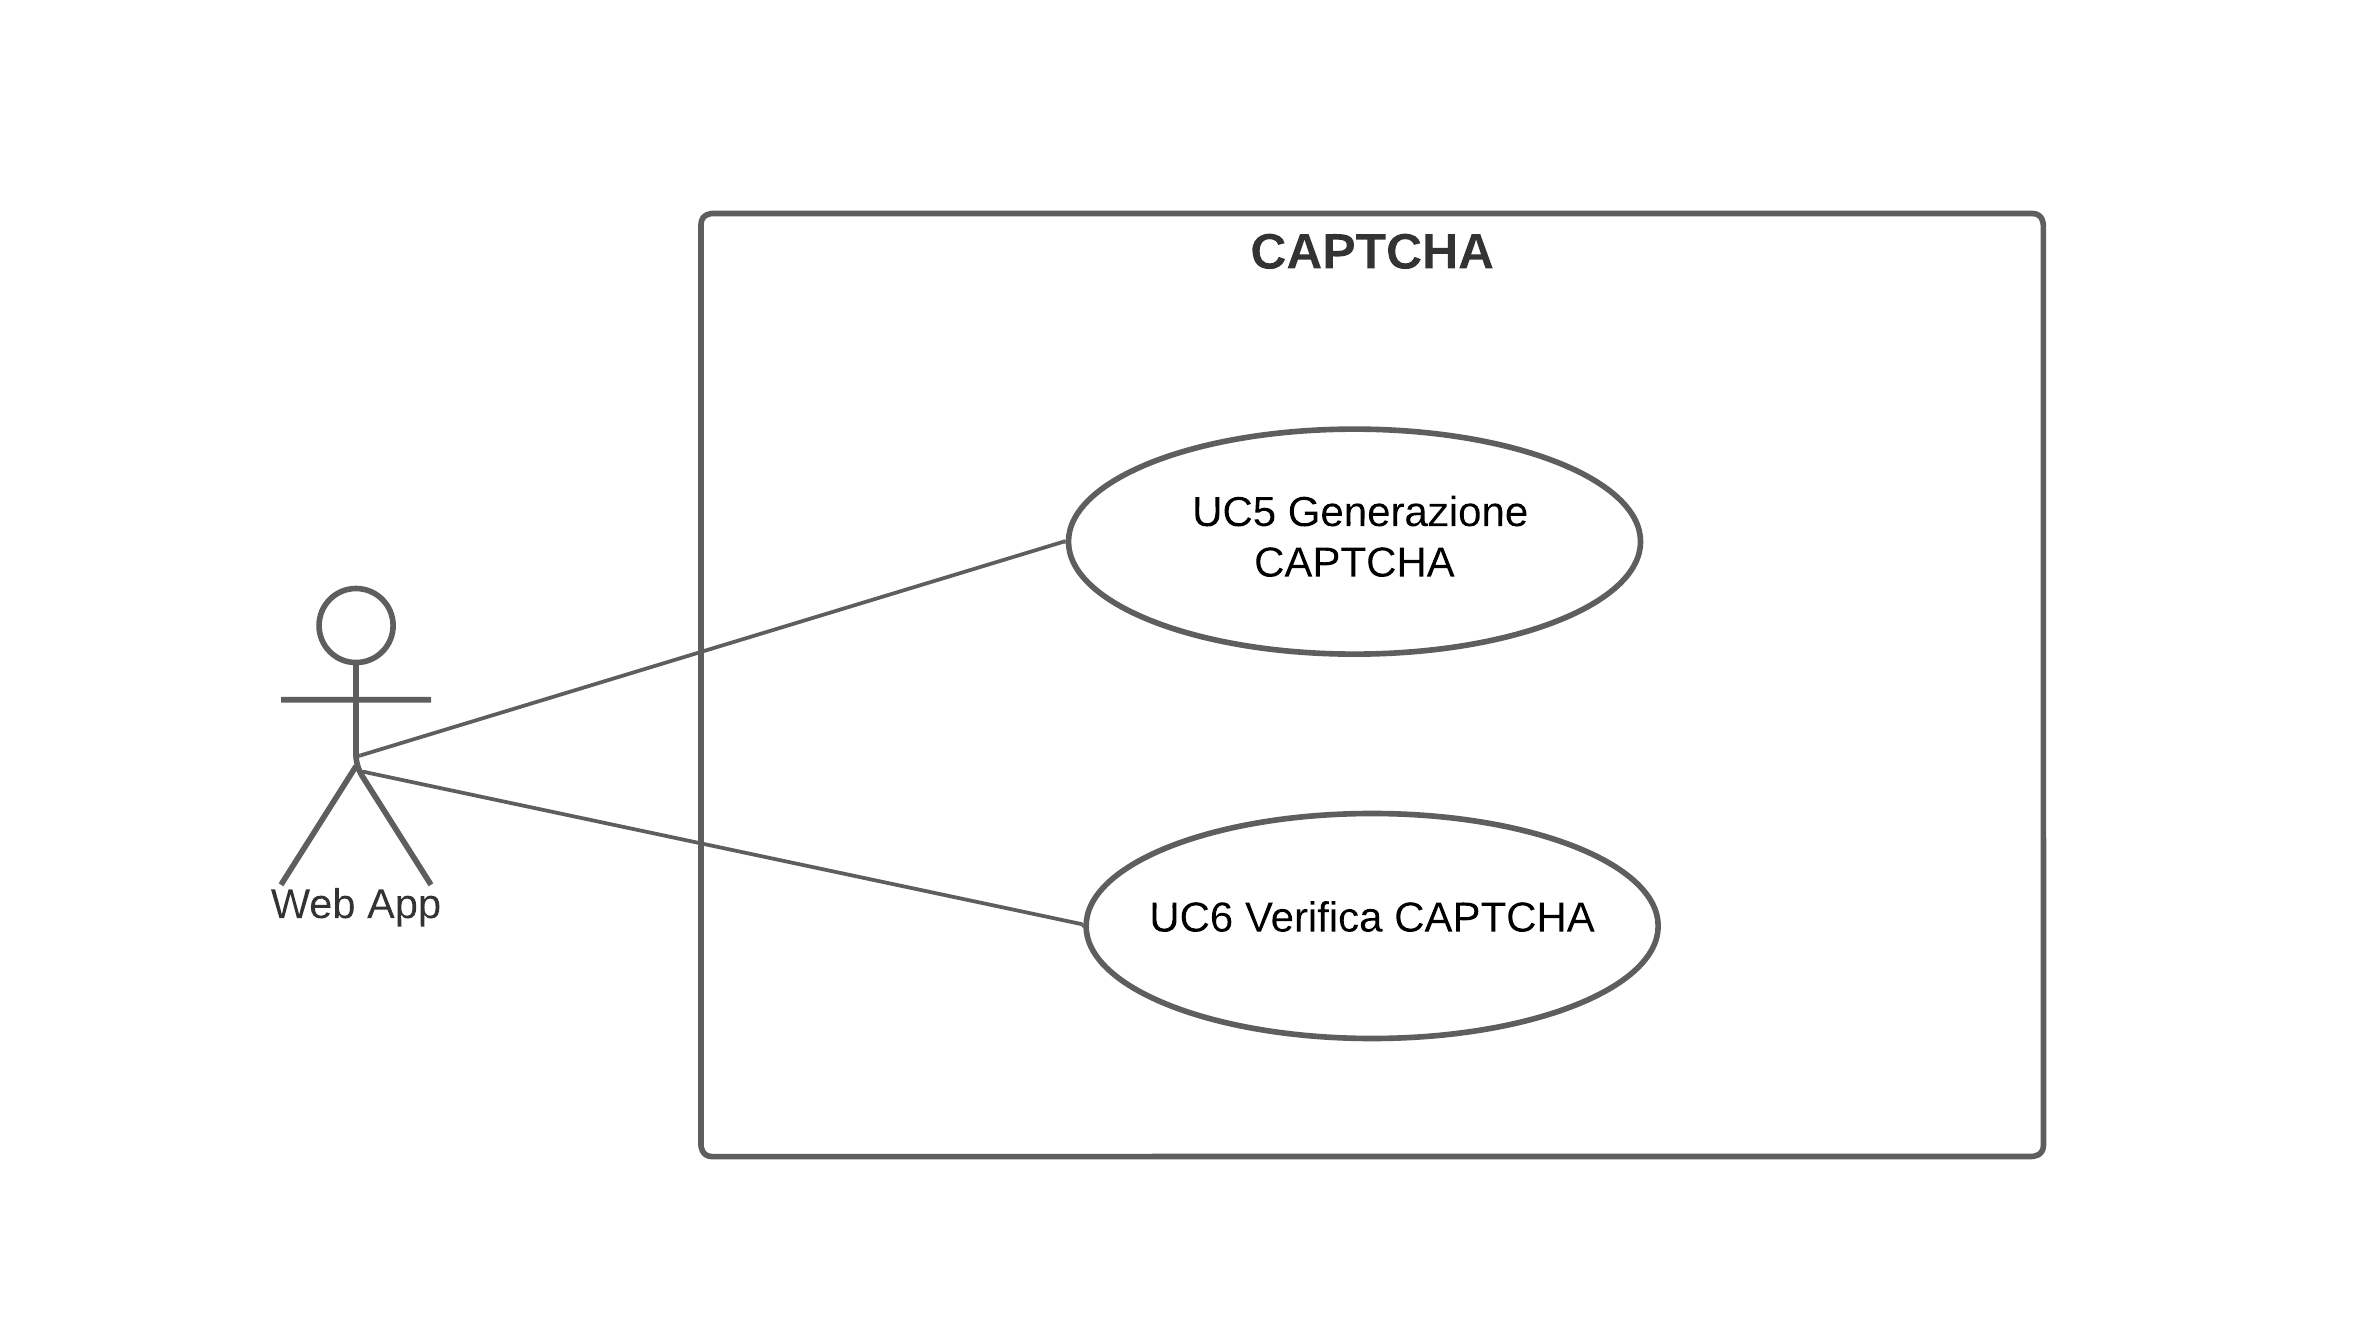
\includegraphics[scale=0.6]{img/captcha.png}
    \caption{CAPTCHA\textsubscript{G}}
\end{figure}

\begin{figure}[H]
    \centering
    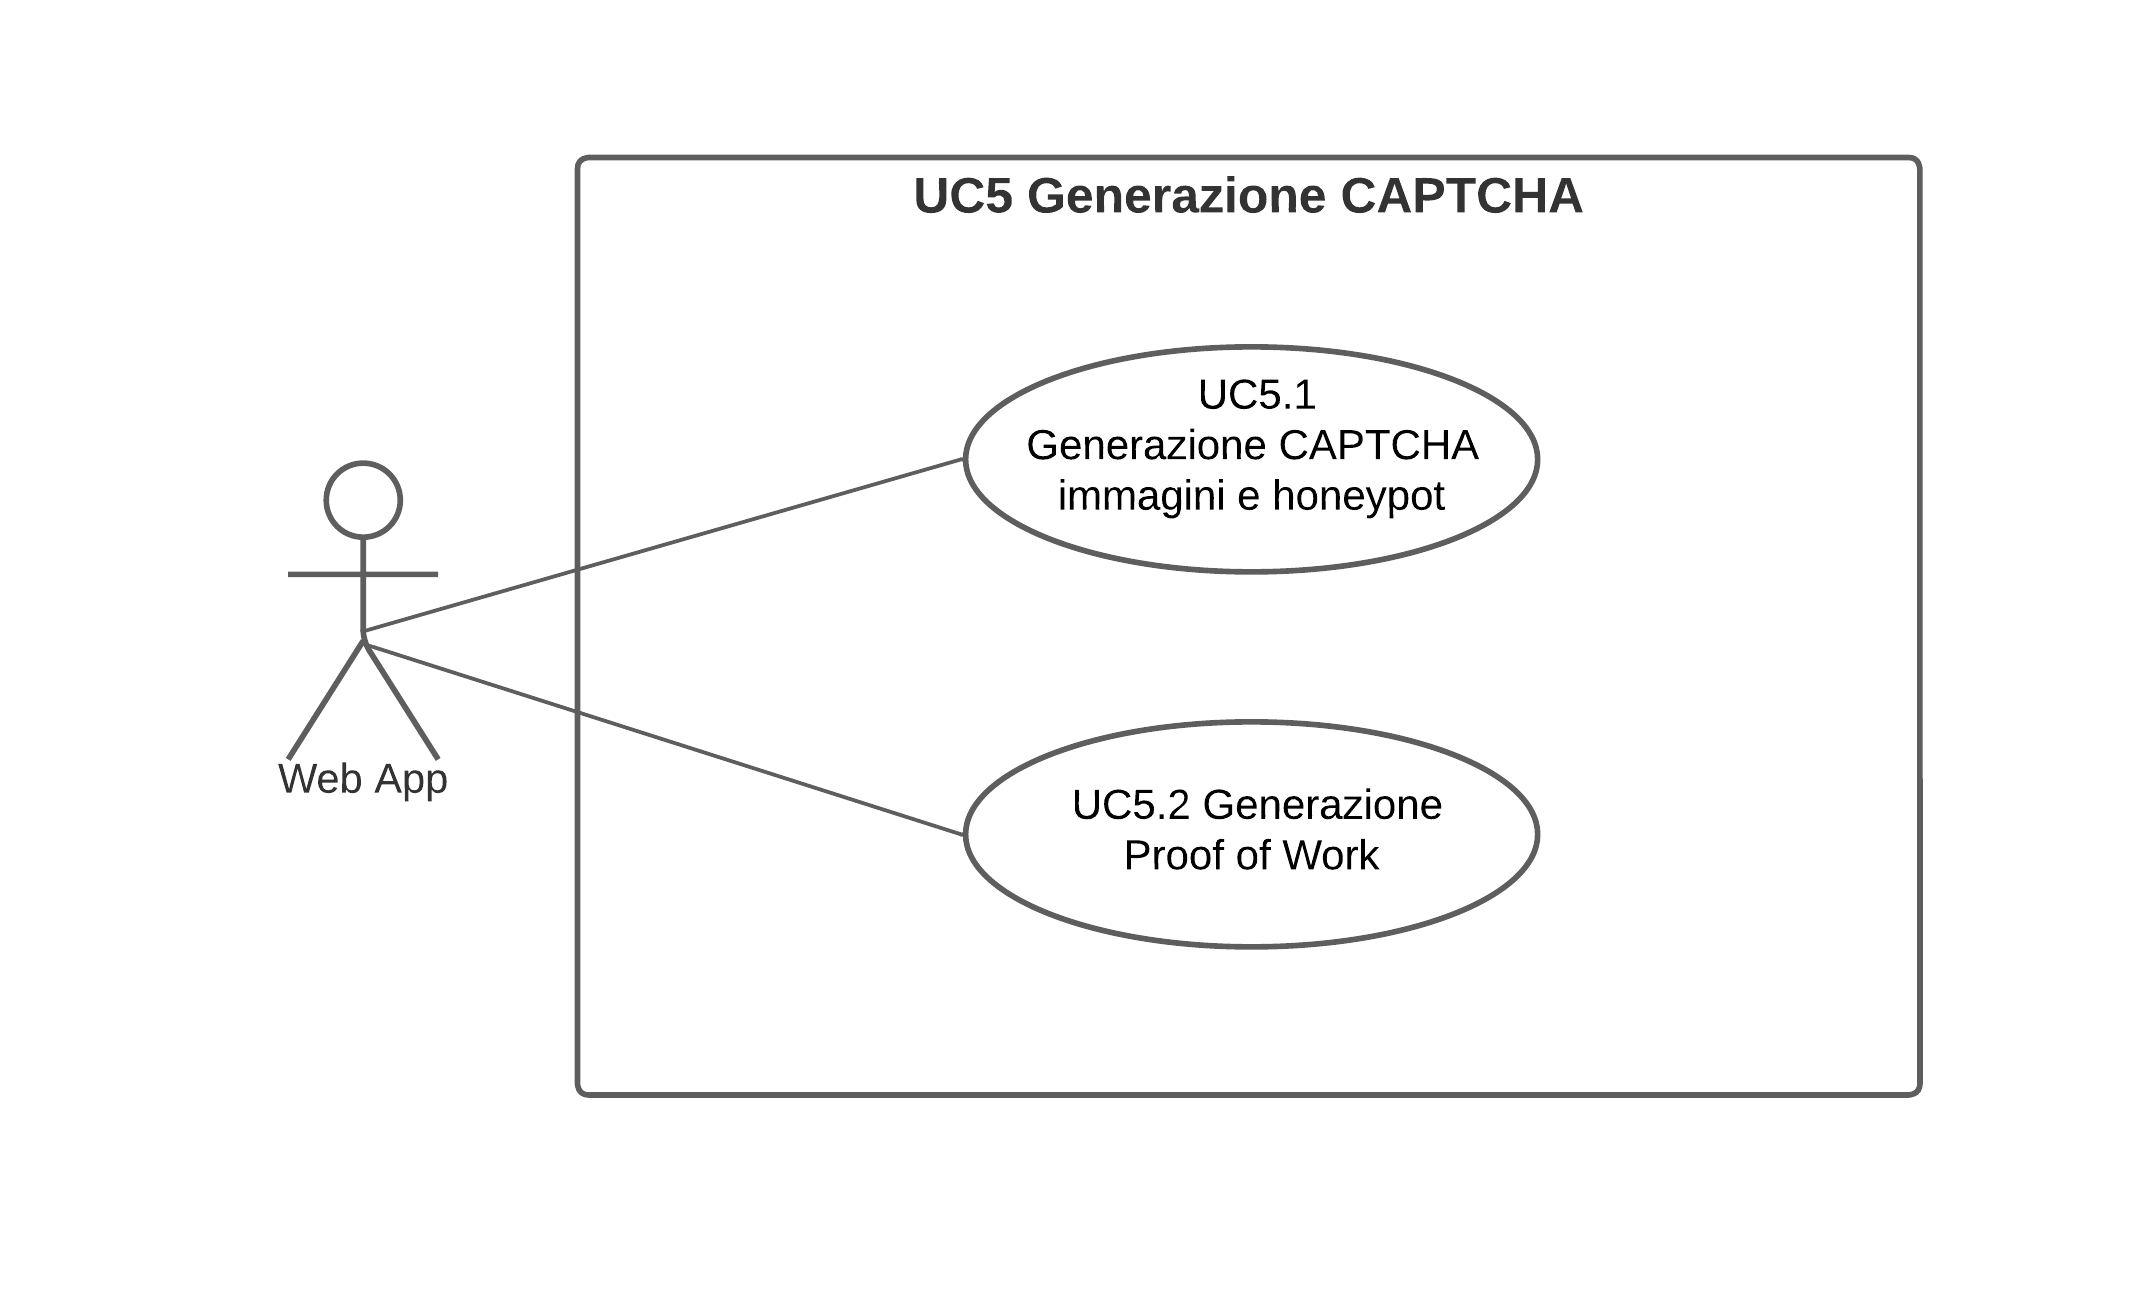
\includegraphics[scale=0.6]{img/generazione.png}
    \caption{UC5 Generazione CAPTCHA\textsubscript{G}}
\end{figure}

\subsubsection{UC5 - Generazione CAPTCHA\textsubscript{G}}
\textbf{Attore primario:} WebApp.\\
\textbf{Precondizioni}: La WebApp richiede la generazione di un CAPTCHA\textsubscript{G}.\\
\textbf{Postcondizioni}: Il CAPTCHA\textsubscript{G} viene generato e restituito alla WebApp.\\

\textbf{Scenario principale}:
\begin{enumerate}
    \item La WebApp richiede la generazione di un CAPTCHA\textsubscript{G};
    \item Il CAPTCHA\textsubscript{G} immagini viene generato utilizzando le immagini presenti nel database interno, assieme ad un'immagine aggiuntiva che funge da honeypot\textsubscript{G} [UC5.1];
    \item Viene generato il Proof of Work [UC5.2];
    \item Il CAPTCHA\textsubscript{G} viene restituito alla WebApp.
\end{enumerate}

\paragraph{UC5.1  - Generazione CAPTCHA\textsubscript{G} immagini}
\textbf{Attore primario:} WebApp.\\
\textbf{Precondizioni}: La WebApp richiede la generazione del CAPTCHA\textsubscript{G} immagini.\\
\textbf{Postcondizioni}: Viene generato il CAPTCHA\textsubscript{G} immagini.\\

\textbf{Scenario principale}:
\begin{enumerate}
    \item La WebApp richiede la generazione del CAPTCHA\textsubscript{G} immagini;
    \item Viene creato il CAPTCHA\textsubscript{G} immagini assieme all'immagine aggiuntiva che funge da honeypot.
\end{enumerate}

\paragraph{UC5.2  - Generazione proof of work\textsubscript{G}}
\textbf{Attore primario:} WebApp.\\
\textbf{Precondizioni}: La WebApp richiede la generazione del proof of work\textsubscript{G}.\\
\textbf{Postcondizioni}: Viene generato il proof of work\textsubscript{G}.\\

\textbf{Scenario principale}:
\begin{enumerate}
    \item La WebApp richiede la generazione del proof of work\textsubscript{G};
    \item Viene creato il proof of work\textsubscript{G} per il CAPTCHA\textsubscript{G}.
\end{enumerate}

\begin{figure}[H]
    \centering
    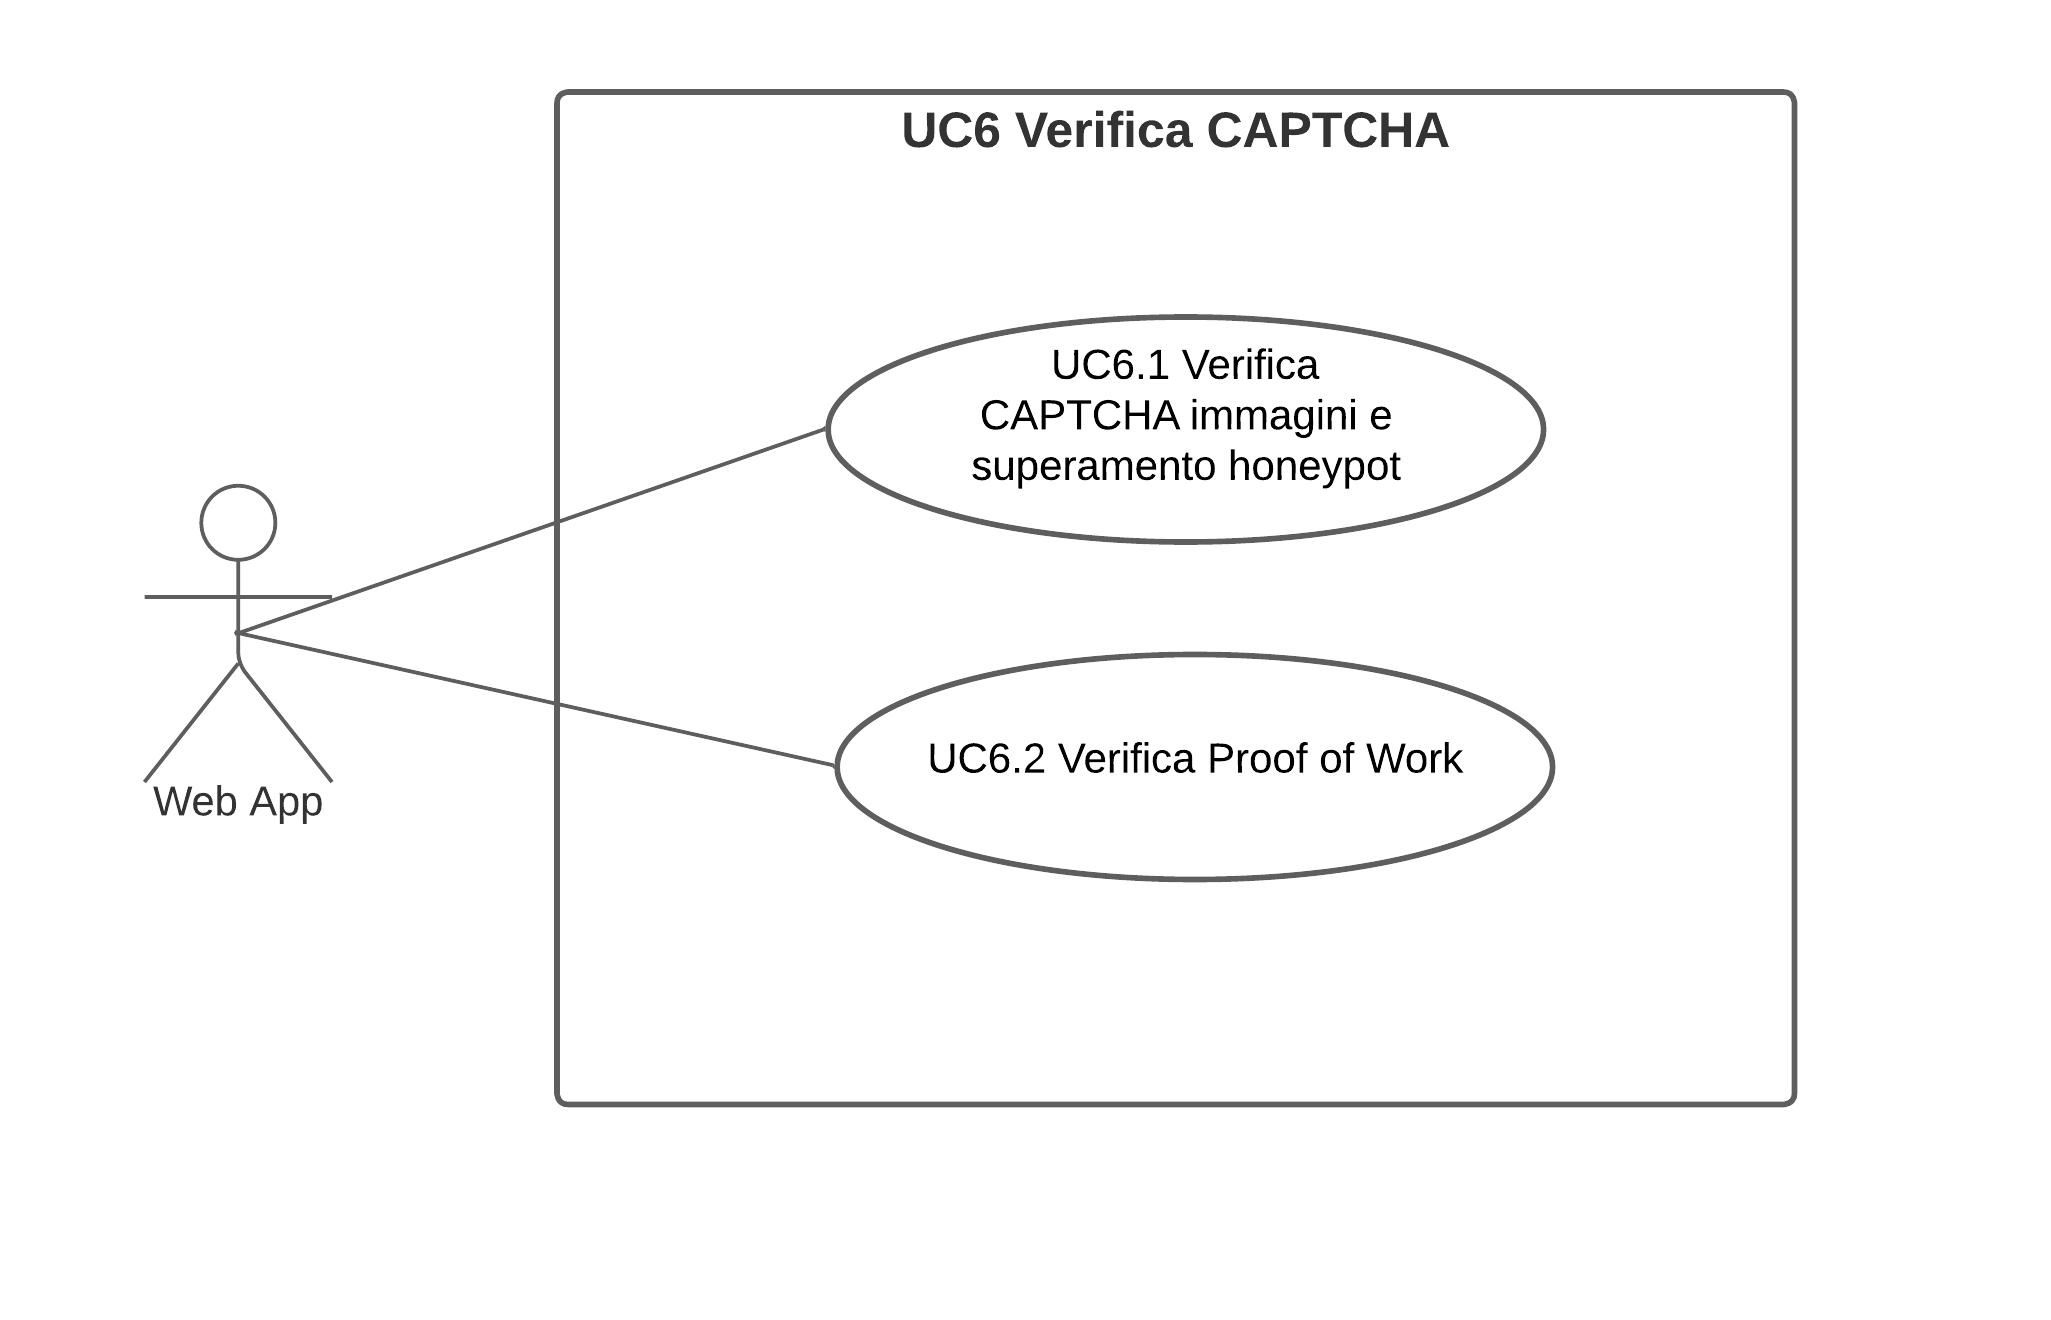
\includegraphics[scale=0.6]{img/verifica.png}
    \caption{UC6 Verifica CAPTCHA\textsubscript{G}}
\end{figure}

\subsubsection{UC6 - Verifica CAPTCHA\textsubscript{G}}
\textbf{Attore primario:} WebApp.\\
\textbf{Precondizioni}: La WebApp richiede la verifica 
 del CAPTCHA\textsubscript{G}.\\
\textbf{Postcondizioni}: Viene data una risposta alla WebApp per indicare se il test CAPTCHA\textsubscript{G} è stato superato o meno.\\

\textbf{Scenario principale}:
\begin{enumerate}
    \item La WebApp richiede la verifica della corretteza del CAPTCHA\textsubscript{G} compilato;
    \item Viene verificata la correttezza di:
    \begin{itemize}
		\item CAPTCHA\textsubscript{G} immagini e superamento honeypot [UC6.1];
		\item Proof of work\textsubscript{G} [UC6.2].
    \end{itemize}
    \item Viene emesso il risultato booleano\textsubscript{G} e restituito alla WebApp.
\end{enumerate}

\paragraph{UC6.1 - Verifica CAPTCHA\textsubscript{G} immagini e superamento honeypot}
\textbf{Attore primario:} WebApp.\\
\textbf{Precondizioni}: La WebApp richiede la verifica del CAPTCHA\textsubscript{G} immagini.\\
\textbf{Postcondizioni}: Il superamento del CAPTCHA\textsubscript{G} immagini viene verificato.\\

\textbf{Scenario principale}:
\begin{enumerate}
    \item La WebApp richiede la verifica della corretteza del CAPTCHA\textsubscript{G} immagini;
    \item In base alla percentuale di correttezza viene verificato se il CAPTCHA\textsubscript{G} immagini è stato superato o meno, e che l'honeypot sia stato superato.
\end{enumerate}

\paragraph{UC6.2 - Verifica proof of work\textsubscript{G}}
\textbf{Attore primario:} WebApp.\\
\textbf{Precondizioni}: La WebApp richiede la verifica del superamento del Proof of Work\textsubscript{G}.\\
\textbf{Postcondizioni}: Il superamento del proof of work\textsubscript{G} viene verificato.\\

\textbf{Scenario principale}:
\begin{enumerate}
    \item La WebApp richiede la verifica del superamento del Proof of Work\textsubscript{G};
    \item L'esecuzione dei calcoli richiesti viene verificata sulla base di quanto fornito dalla WebApp come soluzione.
\end{enumerate}
